\href{/bird/1.jpg}{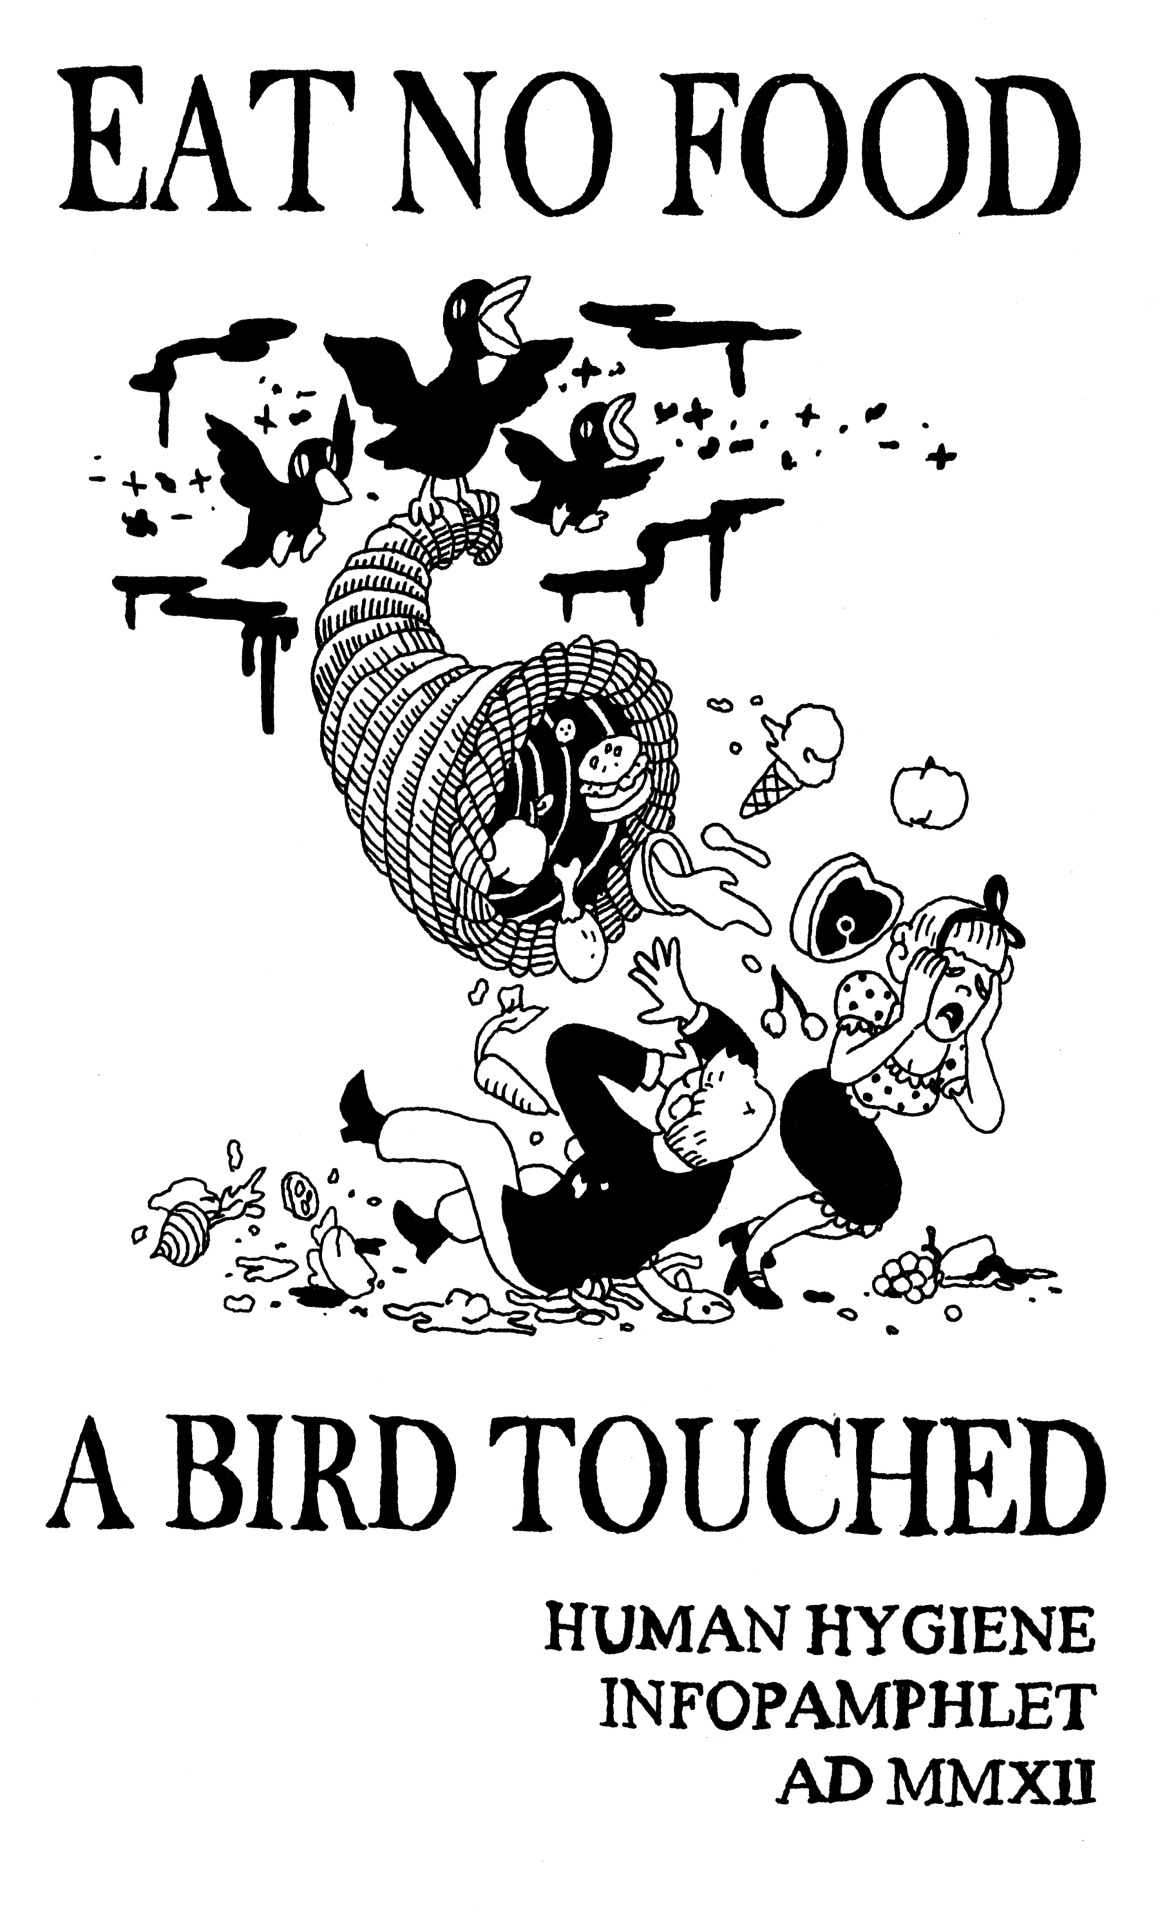
\includegraphics{/bird/1.jpg}}

\begin{verbatim}
Is this a thing for Imgur?  Most certainly not!  It's perfect for shouting into a vasty nothingness, though.  It's just One Of Those Things.  I'd say votes don't matter, since they don't, but Lord knows I'll be back to check on this at some point.  If nothing else, maybe folks with similar experiences will have info, hopes, and thoughts to add.
\end{verbatim}

\href{/bird/2.jpg}{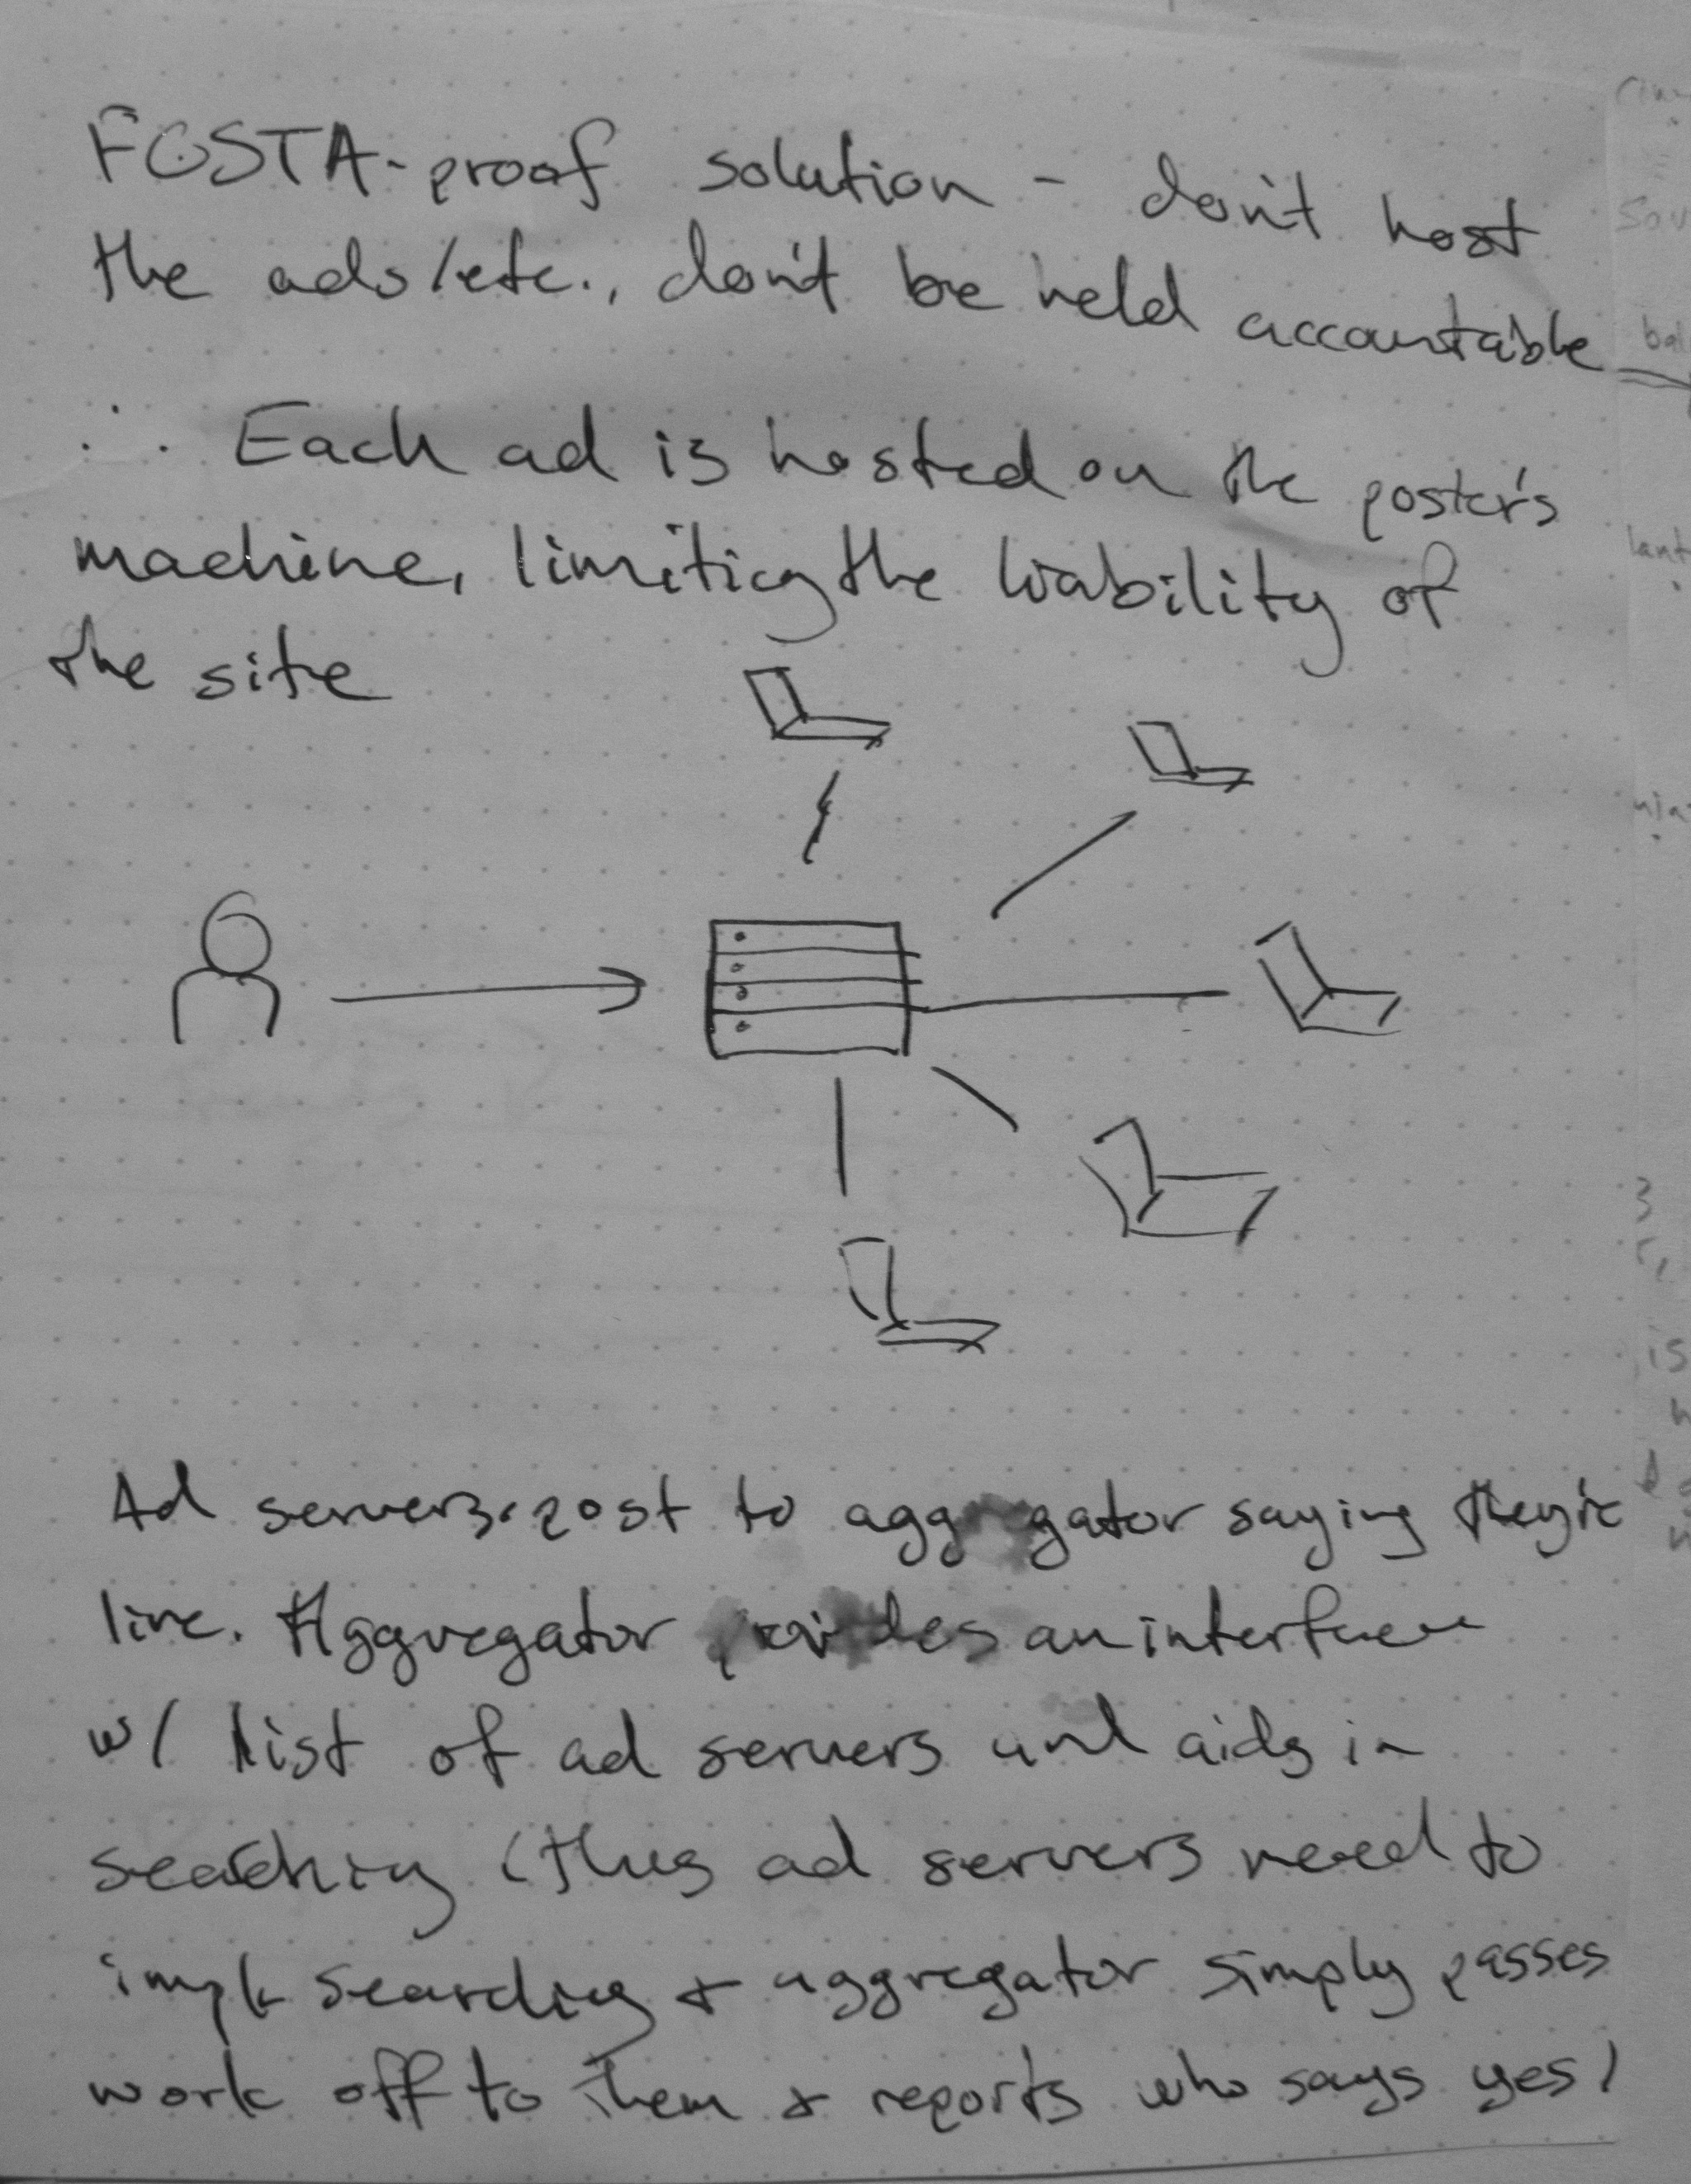
\includegraphics{/bird/2.jpg}}

\begin{verbatim}
This, er...human hygiene infopamphlet strongly evokes the sensation of the destabilization that comes along with going off of antipsychotics (see: http://imgur.com/a/vtulA ).  There’s a certain type of magical, ritualistic thinking that comes with the (near-)psychosis of withdrawal.  The kind that comes on you like a compulsion, or like your gag reflex being triggered, and makes you feel like your skin no longer fits.
\end{verbatim}

\href{/bird/3.jpg}{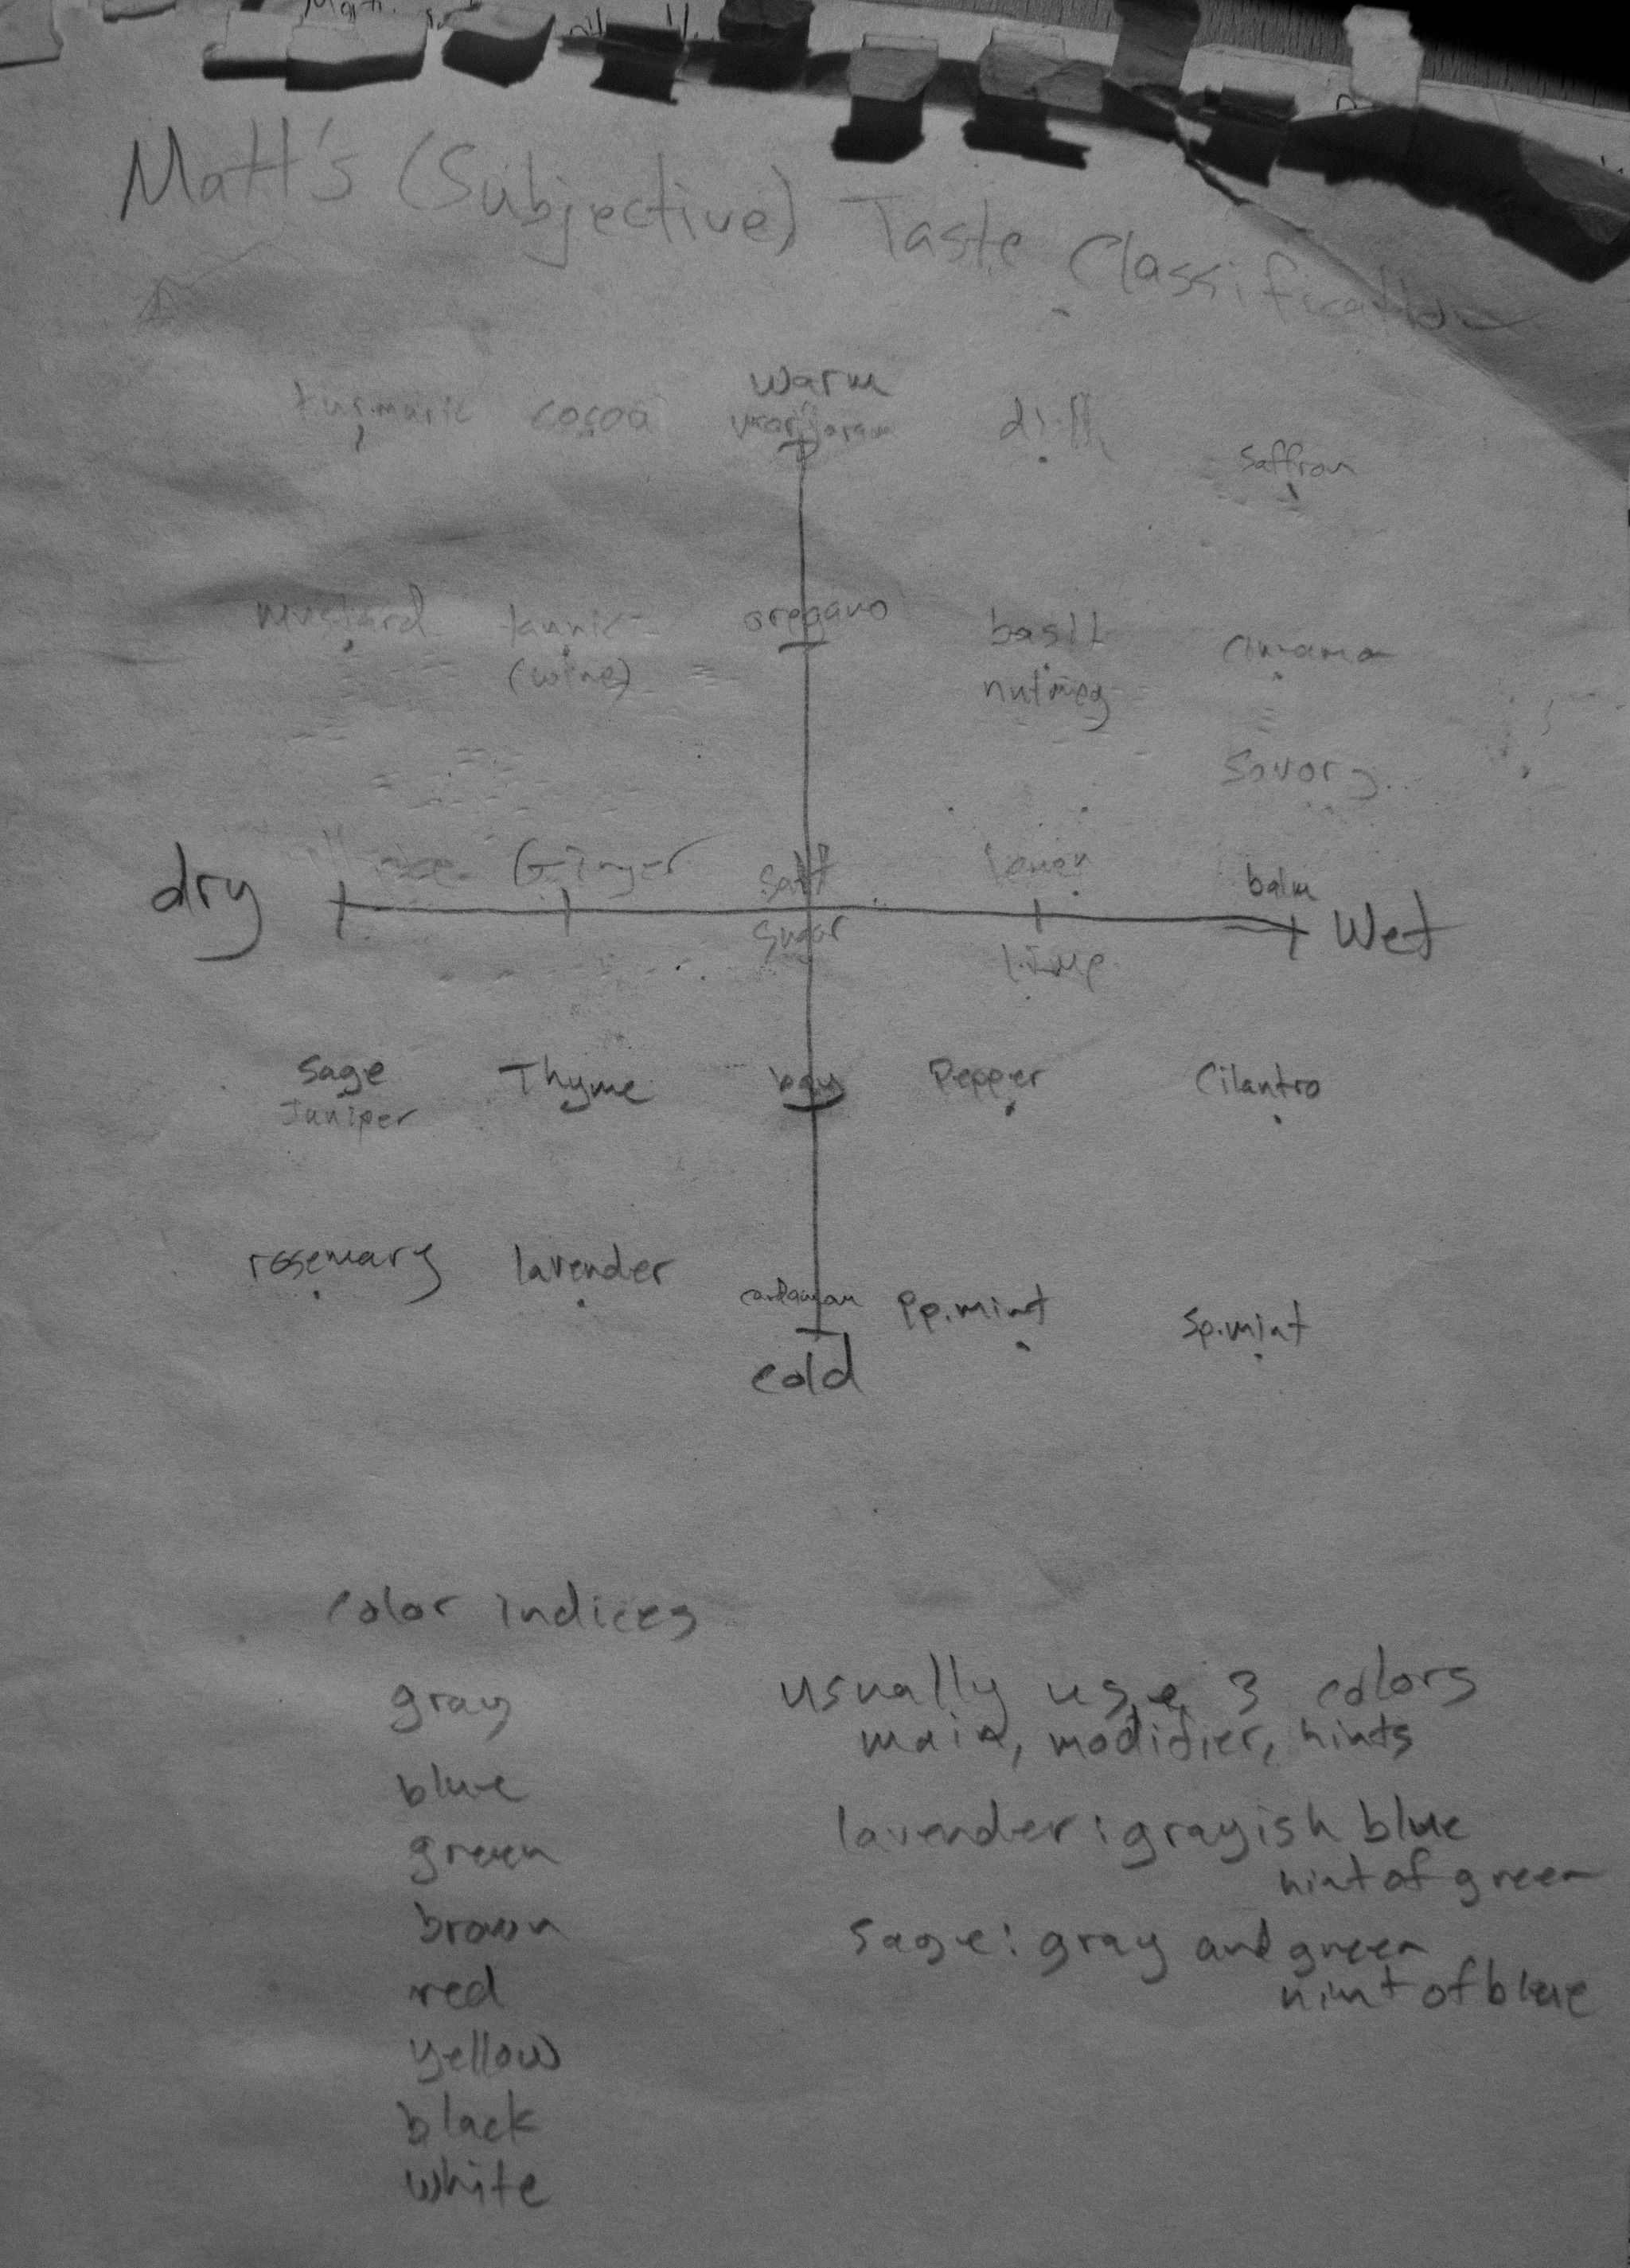
\includegraphics{/bird/3.jpg}}

\begin{verbatim}
For me, it’s frequently about birds.  For a long while, it was geese.  A goose is dumb. A thousand geese darkening the horizon is a portent. Mindless honking, individually directionless, collectively unstoppable.  A goose is tasty. Geese taste like horror. Acrid tang of ill omens.  Or so it felt at the time.

Then it was owls. It was my duty to think about owls, to encourage others to think about owls. In and of themselves, owls are alright, kind of a take-it-or-leave-it bird, but one must think about them, because the consequences of not thinking about them are beyond imagining.  Or so it felt at the time.

And for a bit, it was incantations.  “Get fucked,” I’d tell the clouds.  I’d tell my thoughts to get fucked, I’d tell sleep to get fucked, I’d tell the tic to get fucked.  I had to.  I couldn’t not.  Or so it felt at the time.
\end{verbatim}

\href{/bird/4.jpg}{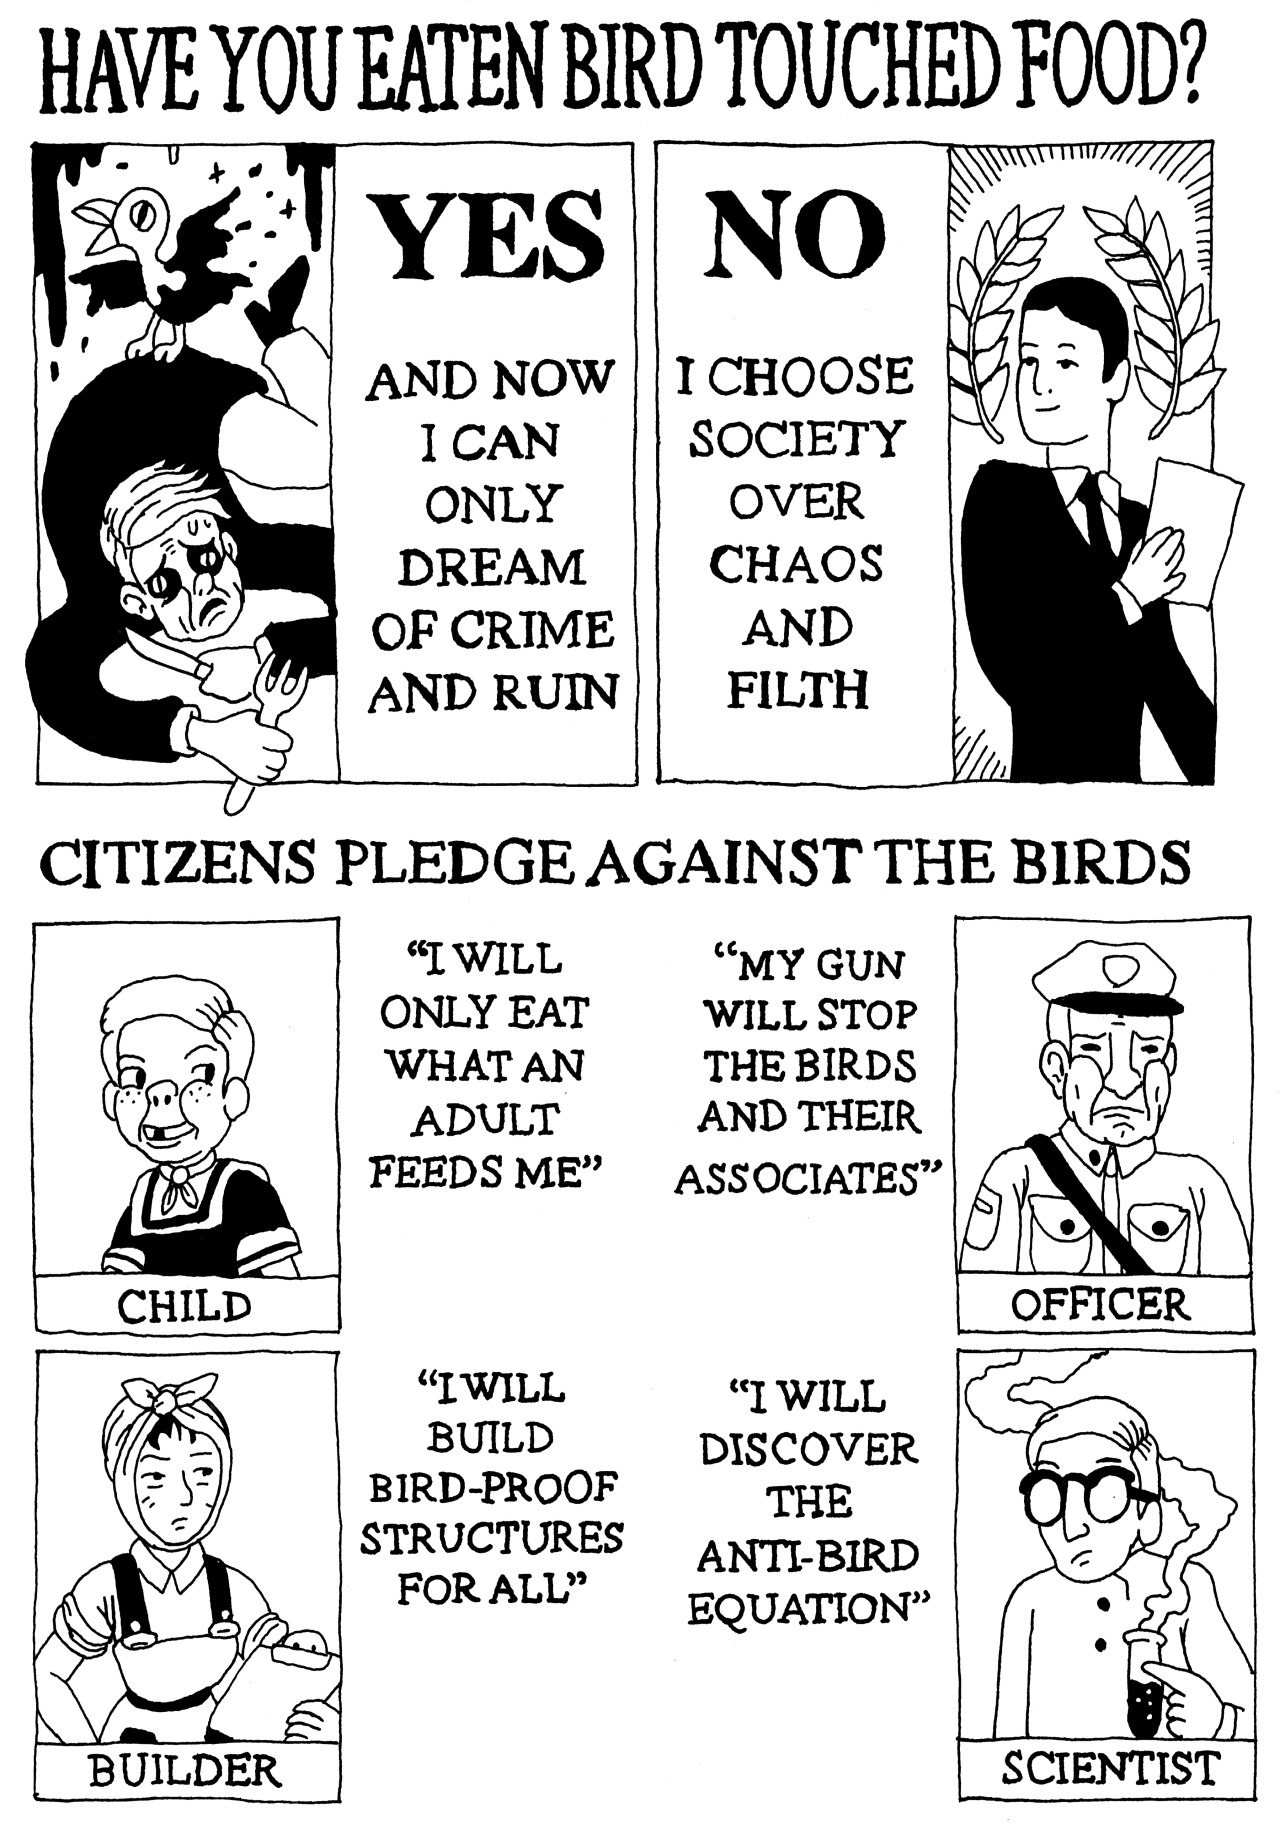
\includegraphics{/bird/4.jpg}}

\begin{verbatim}
Birds and incantations, it turns out, are common in magical thinking and intrusive thoughts, as well as grids, parallel lines, and food.  The comic is a prime example of that.  There are aspects of OCD, sure, but it’s beyond just the obsessions and the compulsions, it’s the way that that is expressed in ritual and dire need, the fact that one cannot bear the consequences of NOT performing the ritual.  There’s nothing wrong with ritual or magical thinking, nor even birds, incantations, grids, or food.  The problem lies in when those are forced on you by your hindbrain until you’re sick.
\end{verbatim}

\href{/bird/5.jpg}{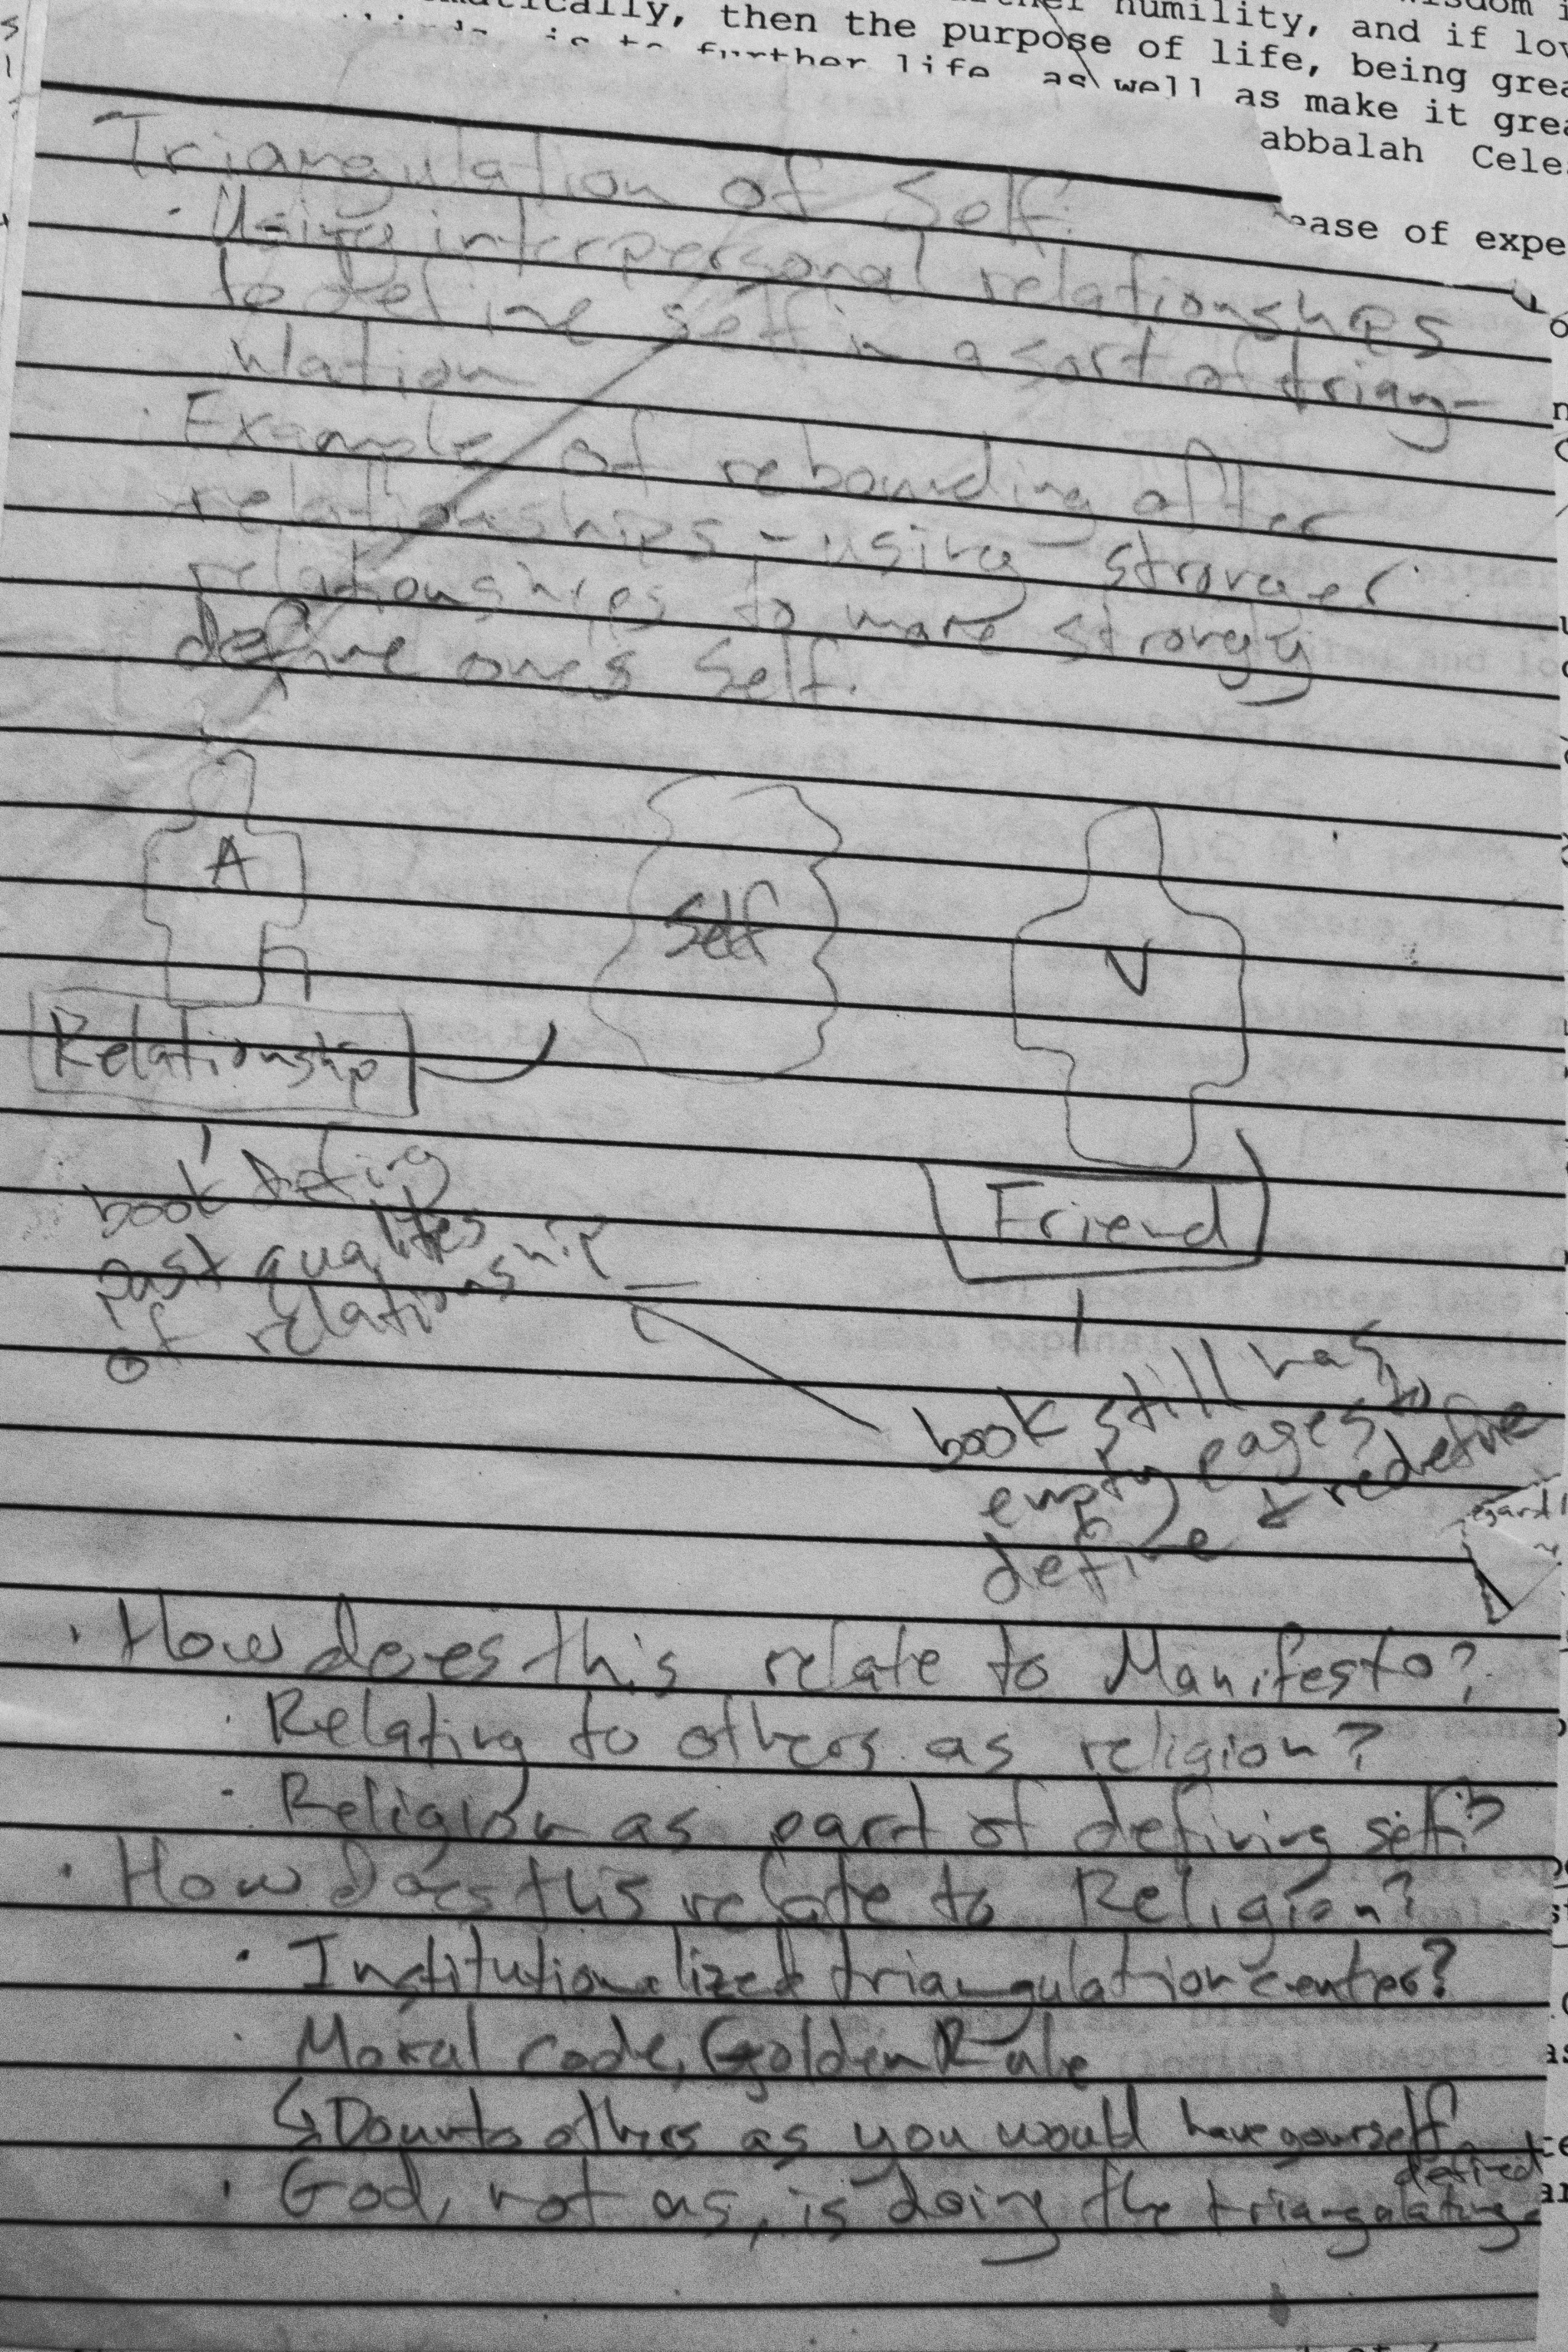
\includegraphics{/bird/5.jpg}}

\begin{verbatim}
A friend calls it ‘bruise vision’, and while I can’t explain why, that’s 100% accurate.
\end{verbatim}

\href{/bird/6.jpg}{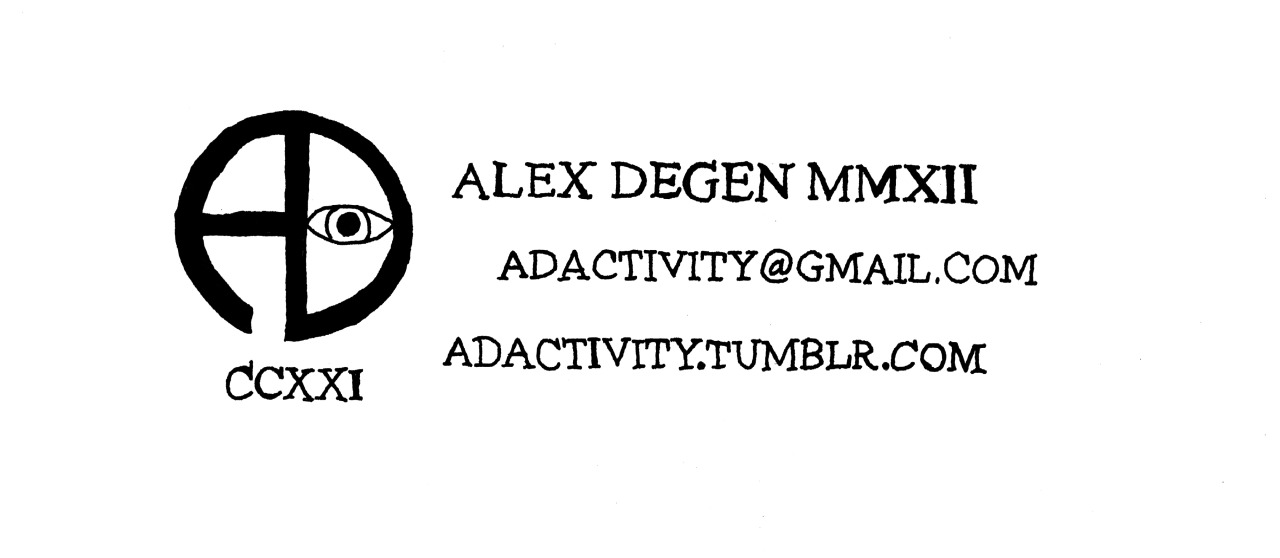
\includegraphics{/bird/6.jpg}}

\begin{verbatim}
I couldn't create this sort of thing, so I'm glad that someone did for me.  Here's the original source: http://adactivity.tumblr.com/post/73552347250/here-are-the-raw-images-which-make-up-the-eat-no  - support artists doing neat things!  And take care of yourselves :)
\end{verbatim}
